\section{Teoria dos Números}
1- Número de subconjuntos de um conjunto é $2^n$, sendo n o número de elementos do conjunto.
\subsection{Exponenciação binária}
Queremos calcular um número $a^x$, podemos fazer isso em complexidade $O(logx)$, utilizando o seguinte algoritmo:
\begin{verbatim}
    long long power(long long base, long long exp) {
        long long result = 1;
    
        while (exp > 0) {
            if (exp % 2 == 1) {
                result *= base;
            }
            base *= base;
            exp /= 2;
        }
    
        return result;
    }

\end{verbatim}
\subsubsection{Exponenciação binária modular}
\par Podemos querer realizar operaçõs de exponenciais grandes, mod algum primo grande. Para isso (REVISAR ESTE CODIGO):
\begin{verbatim}
    // P é o primo grande em questão (i.e. whatsapp 998244353)
    long long power(long long base, long long exp) {
        long long result = 1;
    
        while (exp > 0) {
            if (exp % 2 == 1) {
                result *= base;
                result %= P;
            }
            base *= base;
            base %= P;
            exp /= 2;
        }
    
        return result;
    }
\end{verbatim}
\subsection{Aritmética modular}
 Propriedades:
 \begin{itemize}
     \item $(a + b + c) mod(n) = ((a + b) mod(n) + c) mod(n)$
     \item $(a - b) mod(n)$
        \par Esta operação tem um problema, pois seu valor pode ser negativo, para contornar isso, fazemos: $(a + n - b) mod(n)$. ATENÇÃO: os valores de $a$ e $b$ devem ser válidos, isto é, $a,b\in \left\{0, 1, \cdots, n-1\right\}$.
    \item $(a \cdot b \cdot c) \mbox{ }mod(n) = ((a\cdot b) \mbox{ }mod(n)) \cdot c \mbox{ }mod(n) \cdot$
    \item $(a \cdot b) \mbox{ }mod(n) = ((a\mbox{ }mod(n) \cdot b\mbox{ }mod(n)) \mbox{ }mod(n)$
    \item $(a\cdot b^{-1}) mod(n)$
        \par $b^{-1}$ pode ser lido como o inverso multiplicativo de $b$, ou seja, temos que  \\$b\cdot \frac{1}{b} = 1 \mbox{ }mod(n)$. Se $n$ for primo, todo $a,b$ terá inverso multiplicativo (com exceção de 0).
        \par Pequeno Teorema de Fermat ($a \neq 0$ e $p$ é primo):
        \begin{enumerate}
            \item
            $a^p \equiv a\mbox{ } mod (p)$
            \item $a^{p-1} \equiv 1 mod (p)$
            \item Logo: $a\cdot a^{p-2} \equiv 1 \mbox{ } mod(p)$, portanto: $a^{p-2} \equiv a^{-1}$
            \item Para calcular $a^{p-2}$, utilizar exponenciação binária modular.
        \end{enumerate}
 \end{itemize}

 \subsection{Recorrências lineares}
 \par Em recorrências lineares, é possível encontrar fórmulas fechadas com complexidade $O(\log n)$. Para isto, é utilizada a exponenciação binária de matrizes.
 \par Exemplo: Fibonnacci:
 \begin{center}
     $f_n = f_{n-1} + f_{n-2}, \mbox{ para } n\geq2$.
 \end{center}
 \par Ainda, é possível obter uma transformação linear A de $\mathbb{C}^2$ em $\mathbb{C}^2$ tal que, para todo $n\geq2$,

\begin{equation*}
\mathsf A\begin{pmatrix}
f(n-2)\\
f(n-1)
\end{pmatrix}=
\begin{pmatrix}
f(n-1)\\
f(n)
\end{pmatrix}\,,
\end{equation*}

bastando tomar

\begin{equation*}
\mathsf A=\begin{pmatrix}
0 & 1\\
1 & 1
\end{pmatrix}\,.
\end{equation*}

Assim, indutivamente, temos, para todo $n\geq2$, que

\begin{equation*}
\label{eqfibm}
\mathsf A^{n-1}\begin{pmatrix}
f(0)\\
f(1)
\end{pmatrix}=
\begin{pmatrix}
f(n-1)\\
f(n)
\end{pmatrix}\,.
\end{equation*}

Segue o algoritmo abaixo para o cálculo do n-ésimo número de Fibonacci.

\subsubsection{Multiplicação de matrizes}

\begin{verbatim}    
    vector<vector<int>> matMult(vector<vector<int>>& A, vector<vector<int>>& B) {
    int m = A.size();    // Número de linhas em matrizA
    int n = A[0].size(); // Número de colunas em matrizA
    int p = B[0].size(); // Número de colunas em matrizB

    // Inicialize a matriz de resultado com zeros
    vector<vector<int>> ans(m, vector<int>(p, 0));

    // Realize a multiplicação das matrizes
    for (int i = 0; i < m; i++) {
        for (int j = 0; j < p; j++) {
            for (int k = 0; k < n; k++) {
                ans[i][j] += A[i][k] * B[k][j];
            }
        }
    }

    return ans;
}
\end{verbatim}

\subsubsection{Fibonnaci por exponenciação binária de matrizes}

\begin{verbatim}
    vector<vector<int>> I = {{1,0},{0, 1}}; // matriz identidade

    // exponenciaçào binária de matrizes
    vector<vector<int>> matrixExp(vector<vector<int>> A, int exp){
        if (exp == 0) return I;
        if (exp%2 == 0){
            vector<vector<int>> B = matrixEXp(A, exp/2);
            return matMult(B, B);
        }
        return matMult(A, matrixExp(A, exp-1));
    }

    int fibonnaci(n){
        if (n <= 1) return n;
        vector<vector<int>> B = matrixExp(A, n-1)
        return B[1][1];
    }
\end{verbatim}

\subsection{Fatoração em números primos}
A fatoração em números primos tranforma um número grande em um produto de primos. Por exemplo, 5733, a fatoração pode transformá-lo em 3.3.7.7.13; sendo que cada fator ocupa um índice no vector.
\subsubsection{Fatores repetidos}
\begin{verbatim}
    vector<int> fatoracao (int n){
        vector<int> fatores;
        for (int x=2; x*x<= n; x++)
            while(n%x == 0){
                fatores.push_back(x);
                n/=x;
            }
        if (n>1) fatores.push_back(n);
        return fatores;
    }
\end{verbatim}
\subsubsection{Fatores com expoente}
\begin{verbatim}
    vii fatoracao (int n){
        vii fatores;
        for (int x=2; x*x<= n; x++){
            int exp = 0;
            while(n%x == 0){
                exp++;
                n/=x;
            }
            if (exp > 0)
                fatores.push_back({x,exp});
        }
        if (n>1) fatores.push_back({n,1});
        return fatores;
    }
\end{verbatim}
\subsubsection{Número de Fatores Primos}
\begin{verbatim}
int nFatores (int n){
    for (int x=2; x*x<= n; x++){
        while(n%x == 0){
            n/=x;
            ans++;
        }
    }
    if (n>1) ans++;
    return ans;
}
\end{verbatim}

\subsubsection{Número de Fatores Primos Distintos}
\begin{verbatim}
int nFatoresDistintos (int n){
    int ans = 0;
    for (int x=2; x*x<= n; x++){
        int exp = 0;
        while(n%x == 0){
            exp++;
            n/=x;
        }
        if (exp > 0)
            ans++;
    }
    if (n>1) ans++;
    return ans;
}
\end{verbatim}
\subsubsection{Quantidade de Divisores}
Algoritmo em O(n^1/2)
\begin{verbatim}
    int countDivisors(int x){ 
    int answer = 0; 
    for (int i = 1; i <= sqrt(x); i++) { 
        if (x % i == 0) { 
            if (x / i == i) {answer++;}        
            else { answer = answer + 2; }   
        } 
    } 
    return answer; 
} 

\end{verbatim}
\subsubsection{Soma dos Divisores}
\begin{verbatim}
    int somaDivisores(int n){
        int ans = 1;
        for (int i = 2; i <= n; i+=2){
            int exp = 0;
            while(n%i == 0){
                n/=i;
                exp++;
            }
            if (exp > 0){
                int aux = expbin(i, exp+1);
                ans *= ((aux-1)/(i-1));
            }
            if (i == 2) i--;
        }
    }
\end{verbatim}

\subsection{Função totiente}
A função totiente de Euler retorna a quantidade de números menores que $n$ que são coprimos de $n$;
\begin{verbatim}
    int phi(int n){
        int ans = n;
        for (int i = 2; i*i <= n; i++){
            if (n%i == 0){
                while(n%i == 0)
                    n/=i;
                ans -= ans/i;
            }
        }
        if (n > 1) ans -= ans/n;
        return ans;
    }
\end{verbatim}
\subsection{GCD e LCM}
\par Algoritmo de Euclides (atenção para os limites de INT e LL):
\begin{verbatim}
    int gcd(int a, int b){
        if (b == 0) return a;
        return gcd(b, a%b);
    }
    int lcm(int a, int b){
        return (a*b)/gcd(a, b);
    }
\end{verbatim}

\subsection{Crivo de Eratóstenes}
Algoritmo que calcula todos os números primos entre 1..N em complexidade \\
 O(n*log(log n)).
\begin{verbatim}
    
    void sieve(int n){
        vector<bool> prime(n+1, true);
    
        for (int p = 2; p * p <= n; p++) 
            if (prime[p] == true) 
                for (int i = p * p; i <= n; i += p)
                    prime[i] = false;
            
        
    }
\end{verbatim}

\subsection{Progressões}
    Segue-se abaixo algumas propriedades e equações para o cálculo de 
    progressões aritméticas.
    
    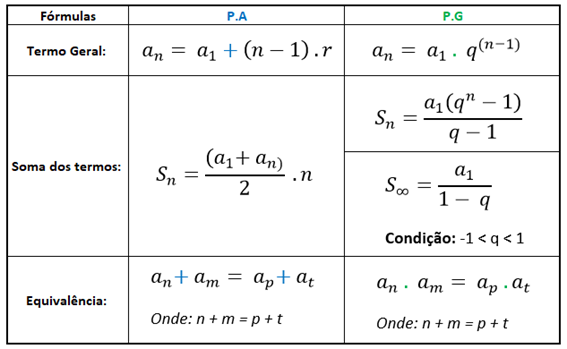
\includegraphics[width=120mm]{7_teoria_dos_numeros/PA_PG.png}

\subsection{Detectar se número é primo}
\begin{verbatim}
    int ehPrimo(int n){
        if (n == 1) return 0;
        if (n == 2) return 1;
        if (n % 2 == 0) return 0;
        for (int i = 3; i*i <= n; i+=2)
            if (n % i == 0) return 0;
        return 1;
    }
\end{verbatim}



\pagebreak
